%
% File acl2013.tex
%
% Contact  navigli@di.uniroma1.it
%%
%% Based on the style files for ACL-2012, which were, in turn,
%% based on the style files for ACL-2011, which were, in turn, 
%% based on the style files for ACL-2010, which were, in turn, 
%% based on the style files for ACL-IJCNLP-2009, which were, in turn,
%% based on the style files for EACL-2009 and IJCNLP-2008...

%% Based on the style files for EACL 2006 by 
%%e.agirre@ehu.es or Sergi.Balari@uab.es
%% and that of ACL 08 by Joakim Nivre and Noah Smith

\documentclass[11pt]{article}
\usepackage{acl2013}
\usepackage{times}
\usepackage{url}
\usepackage{latexsym}
\usepackage{graphicx}
\usepackage{color}
\usepackage{caption}
\usepackage{subcaption}
\usepackage{subfig}



\title{Evaluation of Word Embeddings for Sequence Labelling Tasks}

\author{A Anonymous 
   \\%NICTA / Locked Bag 8001, \\ Canberra ACT 2601, Australia \\
   \\ %The Australian National University\\
   \\ %University of Canberra \\
  \\ % {\tt \small{@nicta.com.au}} \\
\And
  B Anonymous
   \\%NICTA / Locked Bag 8001, \\ Canberra ACT 2601, Australia \\
   \\%The Australian National University\\ \\
   \\ %{\tt \small{@nicta.com.au}} \\
}

\date{2014}

% Max 8 pp.

\begin{document}
\maketitle
\begin{abstract}
XXX
\end{abstract}

\newcommand{\gabi}[1]{\textcolor{blue}{#1}}
\newcommand{\tim}[1]{\textcolor{red}{#1}}
\newcommand{\lizhen}[1]{\textcolor{green}{#1}}
\newcommand{\nss}[1]{\textcolor{magenta}{#1}}

\section{Introduction}
In the last years, distributed word representations
have been applied to several NLP tasks.
Inspired by distributional semantics models, distributed word
representation methods represent each word as a continuous vector, where similar words have a similar vector representation, therefore, capturing the similarity between words.

The resulting vectors can be used as features in many NLP applications and it has been shown that they outperform methods that treats words as atomic units \cite{}.  
Their attractiveness relies in the ability to learn word representations in an unsupervised way, thus directly providing lexical features from big amounts of unlabelled data 
and, therefore, alleviating the cost of human annotations.
It has been also claimed that word embeddings
have the ability to connect out of vocabulary words to known ones.
%, as well known as vocabulary expansion hypothesis. 
Hence, suggesting that word embeddings are a good resource 
for applications that need to be adapted to a certain domain, 
different from the one the application have been tuned for.
For example,...
Another property attribute to word embeddings is their 
capacity to encouraging common behaviour among related in-vocabulary words, for instance...

{\color{red}Short sentence about the architectures}

As with other learning methods, it is well known that
the performance of machine learning algorithms heavily depends on
parameter optimization, the size of the training data used and the applications they target.
For example, \cite{turian2010word} shows that the optimal word embedding dimensions are task specific.
Moreover, there are several word embeddings methods, which used different algorithms and resources. 
Some methods involve feedback from the end task when learning (or fine-tuning) the word representations and others do not. 
Learning algorithm that involves fine-tuning are supposed
to perform better since word representations become
task-specific, at the cost of performing worst for out of vocabulary 
words. But still, there is not systematic comparison between
these two methods. 

%6) How exactly should word representations be incorporated into feature-based sequence tagging models? (May have been answered by the Guo et al. paper.) 
%I believe there is always a better way of doing this, empirical methods as in Guo’s paper or deep sequence neural networks are the ways to go. However, all of them treat the word embeddings trained with different methods in the same way. I conjecture that we should treat them differently based on how they are trained.


In this paper, we perform an extensive evaluation of five word embedding approaches under fixed experiment conditions, and evaluate them over different sequence labelling tasks: POS-tagging, chunking, 
NER and MWE (Multi Word Expression Identification), 
within the following aims:
(i) perform a fair comparison of different word embeddings
algorithms. This includes running different word embeddings algorithms under controlled conditions, for example, use the same training set, the same preprocessing, etc.;
(ii) measure the influence of word embeddings in sequence labeling tasks in semi-supervised settings (fine-tuning);
(iii) systematically compared the usefulness of word embedding versus
unigram features for sequence tagging.
(iv) use word embeddings for MWE. To the best of our knowledge, 
word embeddings have not been used for this task before;


%(i) are word embeddings always better than unigram features? 
%(ii) which word embeddings approach is the best? 
%(iii) to what extend they word embeddings approaches are task specific?
%(iv) how reliable are in labeling out-of-domain data and?

% the conextion between dist. semantics models and sequence taggin. 
%static share hypothesis (in vocabulary words, e.g., individual first names are also rare in the treebank, but tend to cluster together in distributional representations);
%embedding structure hypothesis (e.g., group words by definiteness, like each, this, every, few, most, etc.).




\section{Related Work}
Word embedding learning methods are the new generation of distributional semantics models and have been applied to several 
NLP tasks that we summaries in this section.

\newcite{collobert2011natural} proposed a neuronal network architecture
that learn word embeddings and use them in POS-tagging, chunking, NER and SRL. 
Without specializing their architecture for the mentioned tasks, they achieve close state-of-the-art performance. After including specialized features (e.g., word suffixes for POS-tagging;  Gazzeters for NER, etc.) and other tricks like cascading and ensambling classifiers, achieve competitive state-of-the-art performance.
% they system is very fast too.
Similarly, \newcite{turian2010word} explored the impact of using word
features learned from cluster-based and word embeddings representations
for NER and chunking. 
They conclude that unsupervised word representation improve NER and chunking, and that combining different word representations can further improve the performance.
Word representation from Brown clusters have been also shown to enhance
Twitter POS tagging \newcite{owoputi2013improved}. 

\newcite{Schneider+:2014} presented a MWE analyser that, among other features, used unsupervised word clusters. 
They observed that the clusters were useful for identifying words that usually belong to proper names, which are considered MWE in the data set used. Nevertheless, they mentioned that it is difficult to measure the impact of the word embeddings features, since other features may capture the same information. 
%Further feature engineering should be carry out in order to find out the impact 

Word embeddings have been also used as features for syntactic dependency parsing and constituent parsing. 
\newcite{Bansal+:2014} used word embeddings as features for dependency parsing, which used the syntactic dependency context instead of the linear context in raw text. They found that simple attempts based on discretization of individual word vector dimensions do not improve parsing. Only when performing hierarchical clustering of the continuous word vectors then using features based on the hierarchy, they gain performance. They also pointed out that ensemble of different word embeddings representations improved performance.
Within the same aim, \cite{Andreas:Klein:2014} explores the used of word embeddings for constituency parsing and conclude that the
information they provide might be redundant with the one acquire by a syntactic parser trained with a small amount of data. Others that boost the performance when including word embeddings representations for syntactic parsing includes \cite{Koo:2008,Koo:2010,Haffari:2011,Tratz:2011}.

Word embedding have also been applied to other (non-sequential NLP) tasks such as super-sense tagging \cite{Grave:2013}; grammar induction \cite{Spitkovsky:2011} and semantic task such as semantic relatedness, synonymy detection, concept categorization selection preferences and analogy \cite{baroni:2014}

% Koo, T., Carreras, X., & Collins, M. (2008). Simple semi-supervised dependency parsing. ACL (pp. 595?603).
% Koo et al., 2008; http://cs.nyu.edu/~dsontag/papers/KooEtAl_emnlp10.pdf Dual Decomposition for Parsing with Non-Projective Head Automata - Dependency parsing.

%Haffari et al., 2011; http://www.aclweb.org/anthology/P11-2125 Ensemble of different dependency parsing models, each model corresponding to a different syntactic/semantic word clustering annotation.

% Supersense tagger (Grave et al., 2013) https://hal.inria.fr/hal-00833288/PDF/final-version.pdf



\section{Word Representations}

%The statistics about word occurrences in a corpus is the primary source of information available to all supervised methods for learning word representations.
%Traditionally, words were represented in a vocabulary index, were the is not notion about the similarity between words. 

Distributed word representation methods represent each word as a continuous vector, where similar words have a similar vector representation, therefore, capturing
the similarity between words.

{\color{red}Example}

The estimation of the word vectors can be carry out with different models architectures. We evaluate five different word embeddings learning algorithms, which are the following: 
 
\begin{itemize}
\item[-] Glove \cite{pennington2014glove}
\item[-] Skip-gram \cite{Mikolov13}
\item[-] CBOW \cite{Mikolov13}
\item[-] Neural language model \cite{turian2010word}
\item[-] Brown cluster \cite{Brown92class-basedn-gram}
\end{itemize}

The first four methods were chosen because they are recent
state-of-the-art word embedding methods and because their software is
available. The final method (Brown clusters) was selected as a benchmark word representation, which makes use of hard word clusters rather than a distributed representation.

{\color{red}Discuss here about fundamental differences between the above methods}


\section{Experimental Setup}
We evaluate different learning approaches of word embeddings in four different sequence tagging tasks: POS tagging, chunking, NER and MWE identification.

\subsection{Materials}
It is well known that the choice of a corpora have an important effect in the final accuracy of machine learning algorithms. 
Therefore, each word embedding method was trained with the same corpora (Table \ref{corpus}). The main reason of choosing the corpora 
is that they are publicly available. 

\begin{table}[h]
\begin{center}
\begin{small}
\begin{tabular}{lll}
\hline
\textbf{Data set} & \textbf{Size} & \textbf{Words} \\ \hline
UMBC 	& 48.1GB & 3 billions \\
One Billion 	& 4.1GB & 0.8 billions  \\
Latest wikipedia dump & 49.6GB & 3 billions \\
\end{tabular}
\end{small}
\caption{Corpora used to learn word embeddings}
\label{corpus}
\end{center}
\end{table}

\subsection{Preprocessing}

In order to make the comparison of different word embedding approaches across different applications, we applied the same preprocessing to the data sets used. 
The preprocessing pipeline consist of a sentence splitter, a tokenizer, a POS-tagger and a lemmatizer. The pipeline is built with the UIMA architecture and the DKPro NLP tools. 


\subsection{Hyperparameters tuning}

{\color{red} is this section still valid?}

The performance of learning methods heavily depends on their parameters optimization. 
In order to search for the best hyper-parameters, we look for the shared parameters across methods (methods specific parameters were set to their optimal reported values). The parameters we tuned are the followings:

\begin{small}
\begin{itemize}
\item[-]\textbf{Word vector size}: [25, 50, 100, 200, 400, 800].
\item[-]\textbf{Context window size}: [5, 10, 15].
\item[-]\textbf{Number of clusters}: [250, 500, 1000, 2000, 4000]. 
\end{itemize}
\end{small}

For each task, we split the data into a training set, validation set, and a test set (\ref{datasplit}). The hyper parameters are tuned on the validation set with random search~\cite{bergstra2012random}. To be fair, for each model, we randomly choose 100 hyper parameter combinations and pick up the best one based on its performance on the validation set. Then each model is evaluated in a semi-supervised setting. We start with training models on 10\% of the training data, and evaluate them on the test dataset. Then we incrementally add another 10\% of the training data and evaluate them until all training data is used. We adopt per-word F1 scores as the evaluation metric for all tasks except POS tagging, for which we used per-word accuracy.
In order to evaluate model performance on unknown words, we report also the average F1 scores for the words that do not occur in the training set.


\subsection{Training}
For each task, we feed learned embeddings into the graph transformer trained with sentence tag criterion~\cite{turian2010word}. The graph transformer is equivalent to CRF, if we do not update word embeddings. For all tasks, we train graph transformer with pre-trained word embeddings in the following settings: 

\begin{small}
\begin{itemize}
\item[-] CRF with conventional features.
\item[-] Graph transformer \textit{does not} fine tune embeddings during training.
\item[-] Graph transformer fine tunes the embeddings during training.
\end{itemize}
\end{small}

We also set up experiments to verify that CRF/graph transformer requires different feature design for different kinds of pre-trained word embeddings. One kind of word embeddings is represented by~\cite{bengio2006neural}. It maximises the word sequence likelihood with a model based on a weighted linear combination of word embedding features. Another kind of word embeddings is skip-gram and its variants, which is based on the dot product of two word embeddings. Therefore, we compare at least two ways of representing context word embedding features for each token:

\begin{small}
\begin{itemize}
\item[i] Concatenate word embeddings of context words within a fixed window as context features; 
\item[ii] Concatenate the result of element-wise multiplication of current token embedding and each context word embedding as context features. 
\end{itemize}
\end{small}



\begin{table*}
\begin{small}
\begin{tabular}{lllp{3cm}ll}
\hline
			& \textbf{Training} & \textbf{Validation} & \textbf{Test} & \textbf{Feature space} \\ \hline
\textbf{POS-Tagging} & 0-18 of WSJ & 19-21 of WSJ & 22-24 of WSJ and English Web Treebank & as in~\cite{collobert2011natural} \\
\textbf{Chunking} & WSJ & 1000 sentences WSJ & CoNLL2000 & as~\cite{turian2010word}\\
\textbf{NER} & CoNLL2003 train set & CoNLL2003 dev. set & CoNLL2003 test set and MUC7 & as in~\cite{turian2010word} \\
\textbf{MWE} & 500 documents from & 100 documents from & 123 documents & as in~\cite{mwecorpus}\\
\hline
\label{datasplit}
%\caption{Data split into training, validation and test set for each task}
\end{tabular}
\end{small}
\end{table*}


%\subsection{POS tagging} We could choose one of the options. \subsubsection{Option 1} Almost the same setting as~\cite{collobert2011natural}, except adding one more test set.
% \noindent Training set: 0-18 of WSJ.
% \noindent Validation set: 19-21 of WSJ.
% \noindent Test set: 22-24 of WSJ, and English Web Treebank. We report model performances on these two test sets respectively.
% \noindent Feature space: the same set as in~\cite{collobert2011natural}

% \subsection{Chunking} The same setting as~\cite{turian2010word}\\
% \noindent Training set: WSJ train set.
% \noindent Validation set: Randomly sampled 1000 sentences from the train set for development.
% \noindent Test set: CoNLL2000 test set.
% \noindent Feature space: the same set as in~\cite{turian2010word}

% \subsection{MWE Identification} Training set: randomly sampled 500 documents from Nathana��s corpus. 
% \noindent Validation set: randomly sampled 100 documents from Nathana��s corpus.
% \noindent Test set: remaining 123 documents from Nathana��s corpus..
% \noindent Feature space: the same set as in~\cite{mwecorpus}

%\subsection{Named entity recognition} Training set: CoNLL03 train set.
% \noindent Validation set: CoNLL03 development set.
% \noindent Test set: CoNLL03 test set and MUC7. We report model performances on these two test sets respectively.
% \noindent Feature space: the same set as in~\cite{turian2010word}

\section{Experimental Results and Discussion}



Because we can either update pre-trained word embeddings during training or not, through the evaluation, we want to answer the following questions:
\begin{itemize}
\item How well do different word embeddings perform in all tasks when supervised fine-tuning is \textit{not} performed?
\item How well do different word embeddings perform in all tasks when supervised fine-tuning is performed?
\item How does the size of labeled training data affect the experimental results?
\item How well do the word embeddings perform for unknown words? 
\item How do the key parameters of each word learning algorithms affect the experimental results?
\end{itemize}

%%%%%%%%%%%%%%%%%%%%%%%%%%%%
%%% BESTS
\begin{figure*}
\caption{Best results for each method for POS-Tagging and Chunking}
\centering
\begin{subfigure}{.5\textwidth}
	\centering
    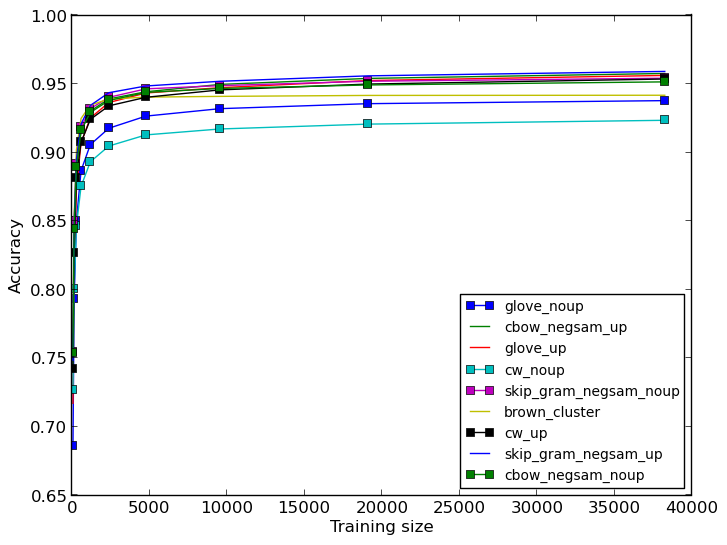
\includegraphics[width=0.8\textwidth]{plots/bestPOS.png}    	
	\label{fig:bestpos}
	\subcaption{POS-Tagging results}	
\end{subfigure}%
\begin{subfigure}{.5\textwidth}
	\centering
    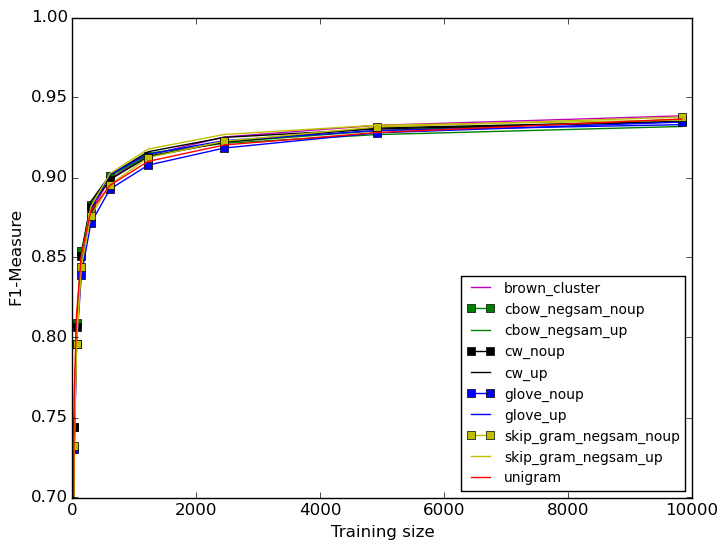
\includegraphics[width=0.8\textwidth]{plots/bestChunking.png}
	\label{fig:bestchunking}
	\subcaption{Chunking results}	
\end{subfigure}
\end{figure*}

\begin{figure*}
\caption{Best results for each method for NER and MWE}
\centering
\begin{subfigure}{.5\textwidth}
	\centering
    	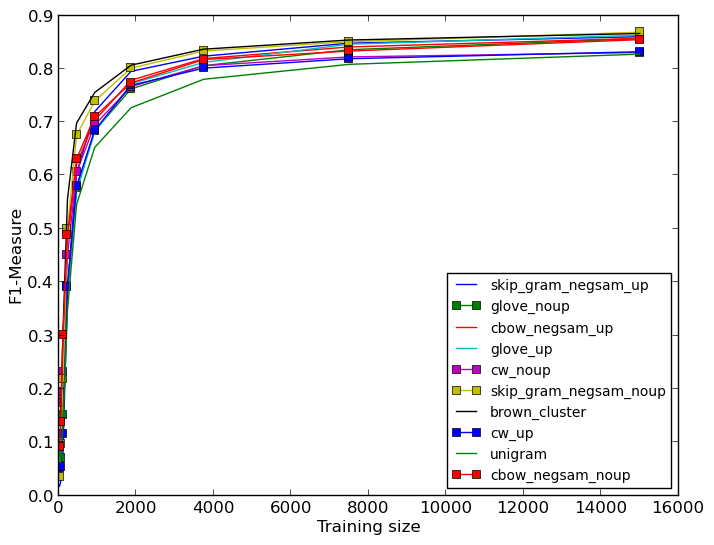
\includegraphics[width=0.8\textwidth]{plots/bestNER.png}
	\subcaption{NER results}	
	\label{fig:bestner}
\end{subfigure}
\begin{subfigure}{.5\textwidth}
	\centering
    	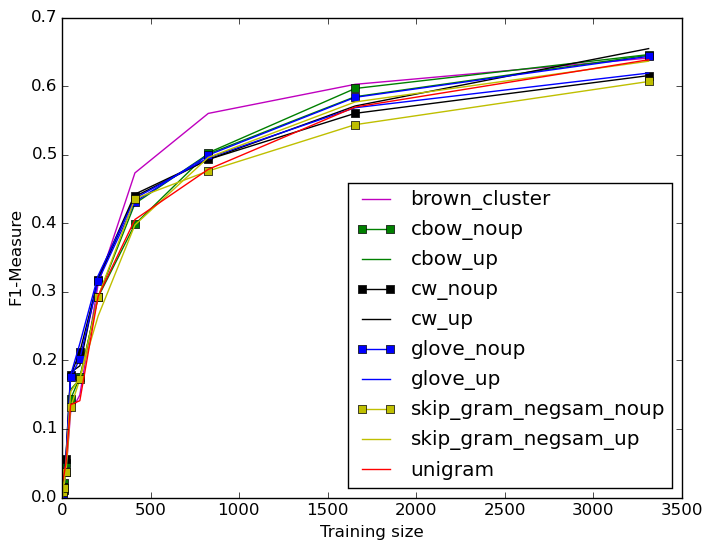
\includegraphics[width=0.8\textwidth]{plots/bestMWE.png}
    \subcaption{MWE results}	
	\label{fig:bestmwe}
\end{subfigure}  	
\end{figure*}  	


%%%%%%%%%%%%%%%%%%%%%%%%%%%%
%%% OUT OF VOC POS

\begin{figure*}
\caption{POS-Tagging out-of-vocabulary-words accuracy for \textit{in-domain} and \textit{out-of-domain} test sets}
\centering
\begin{subfigure}{.5\textwidth}
	\centering
    	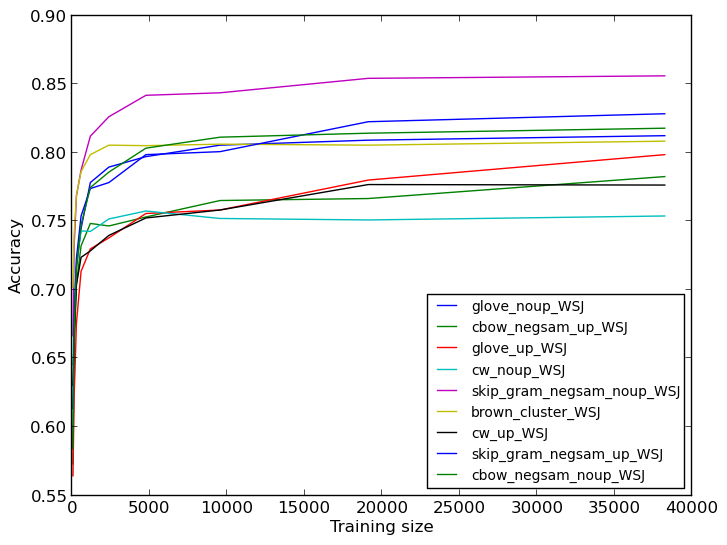
\includegraphics[width=0.8\textwidth]{plots/POSoutOfVocIN.png}
    	\subcaption{\textit{in domain} }
	\label{fig:inpos}
\end{subfigure}
\begin{subfigure}{.5\textwidth}
	\centering
    	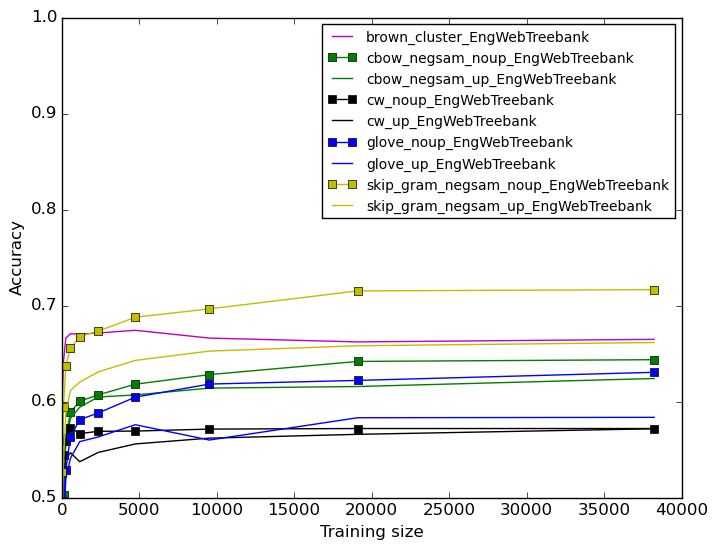
\includegraphics[width=0.8\textwidth]{plots/POSoutOfVocOUT.png}
   	\subcaption{\textit{out-of-domain}}
	\label{fig:outpos}
\end{subfigure}  	
\end{figure*} 

%%%%%%%%%%%%%%%%%%%%%%%%%%%%
%%% OUT OF VOC Chunking: missing result!!!

%%%%%%%%%%%%%%%%%%%%%%%%%%%%
%%% OUT OF VOC NER
\begin{figure*}
\caption{NER out-of-vocabulary-words accuracy for \textit{in-domain} and \textit{out-of-domain} test sets}
\centering
\begin{subfigure}{.5\textwidth}
	\centering
    	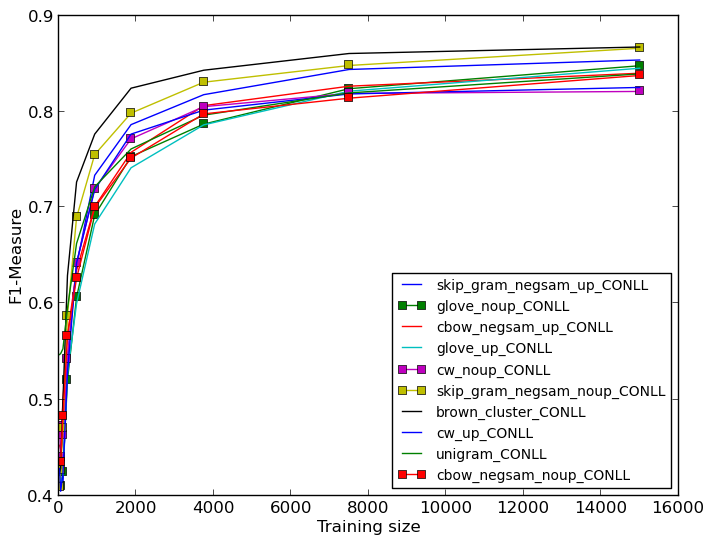
\includegraphics[width=0.8\textwidth]{plots/NERoutOfVocIN.png}
    	\subcaption{\textit{in-domain}}
	\label{fig:inner}
\end{subfigure}
\begin{subfigure}{.5\textwidth}
	\centering
    	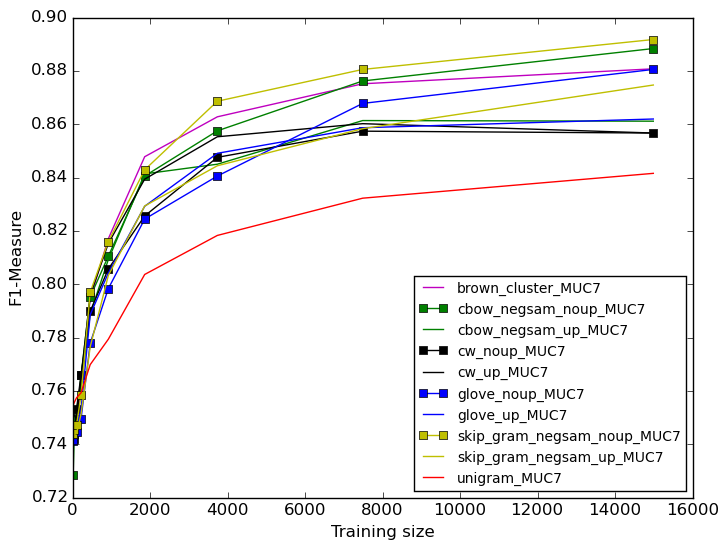
\includegraphics[width=0.8\textwidth]{plots/NERoutOfVocOUT.png}
   	\subcaption{\textit{out-of-domain}}
	\label{fig:outner}
\end{subfigure}  	
\end{figure*}


%%%%%%%%%%%%%%%%%%%%%%%%%%%%
%%% OUT OF VOC MWE
\begin{figure*}
\caption{MWE out-of-vocabulary-words accuracy for \textit{in-domain} test set}
\centering
    	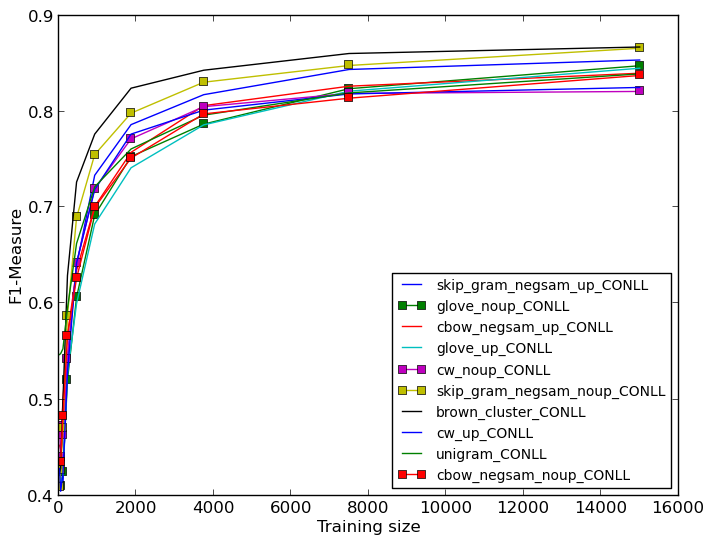
\includegraphics[width=0.5\textwidth]{plots/NERoutOfVocIN.png}    
\label{fig:outmwe}
\end{figure*}

%%%%%%%%%%%%%%%%%%%%%%%%%%%%
%%% OUT OF VOC POS




\section{Conclusion}



\section*{Acknowledgments}

Anonymised\\
Anonymised\\
Anonymised\\
Anonymised\\
Anonymised\\
Anonymised\\

%NICTA is funded by the Australian Government as represented by the Department of Broadband, Communications and the Digital Economy and the Australian Research Council through the ICT Centre of Excellence program.

\bibliographystyle{acl2013}
\bibliography{biblio}

\end{document}

